\documentclass[aspectratio=169,11pt]{beamer}
\usetheme{default}
\setbeamertemplate{navigation symbols}{}
\setbeamercolor{frametitle}{fg=black}
\setbeamerfont{frametitle}{size=\Large,series=\bfseries}
\usepackage{graphicx,booktabs}
\graphicspath{{../report/figures/}}
\begin{document}
\begin{frame}{A world model that learned golf from pixels discovered the walls}
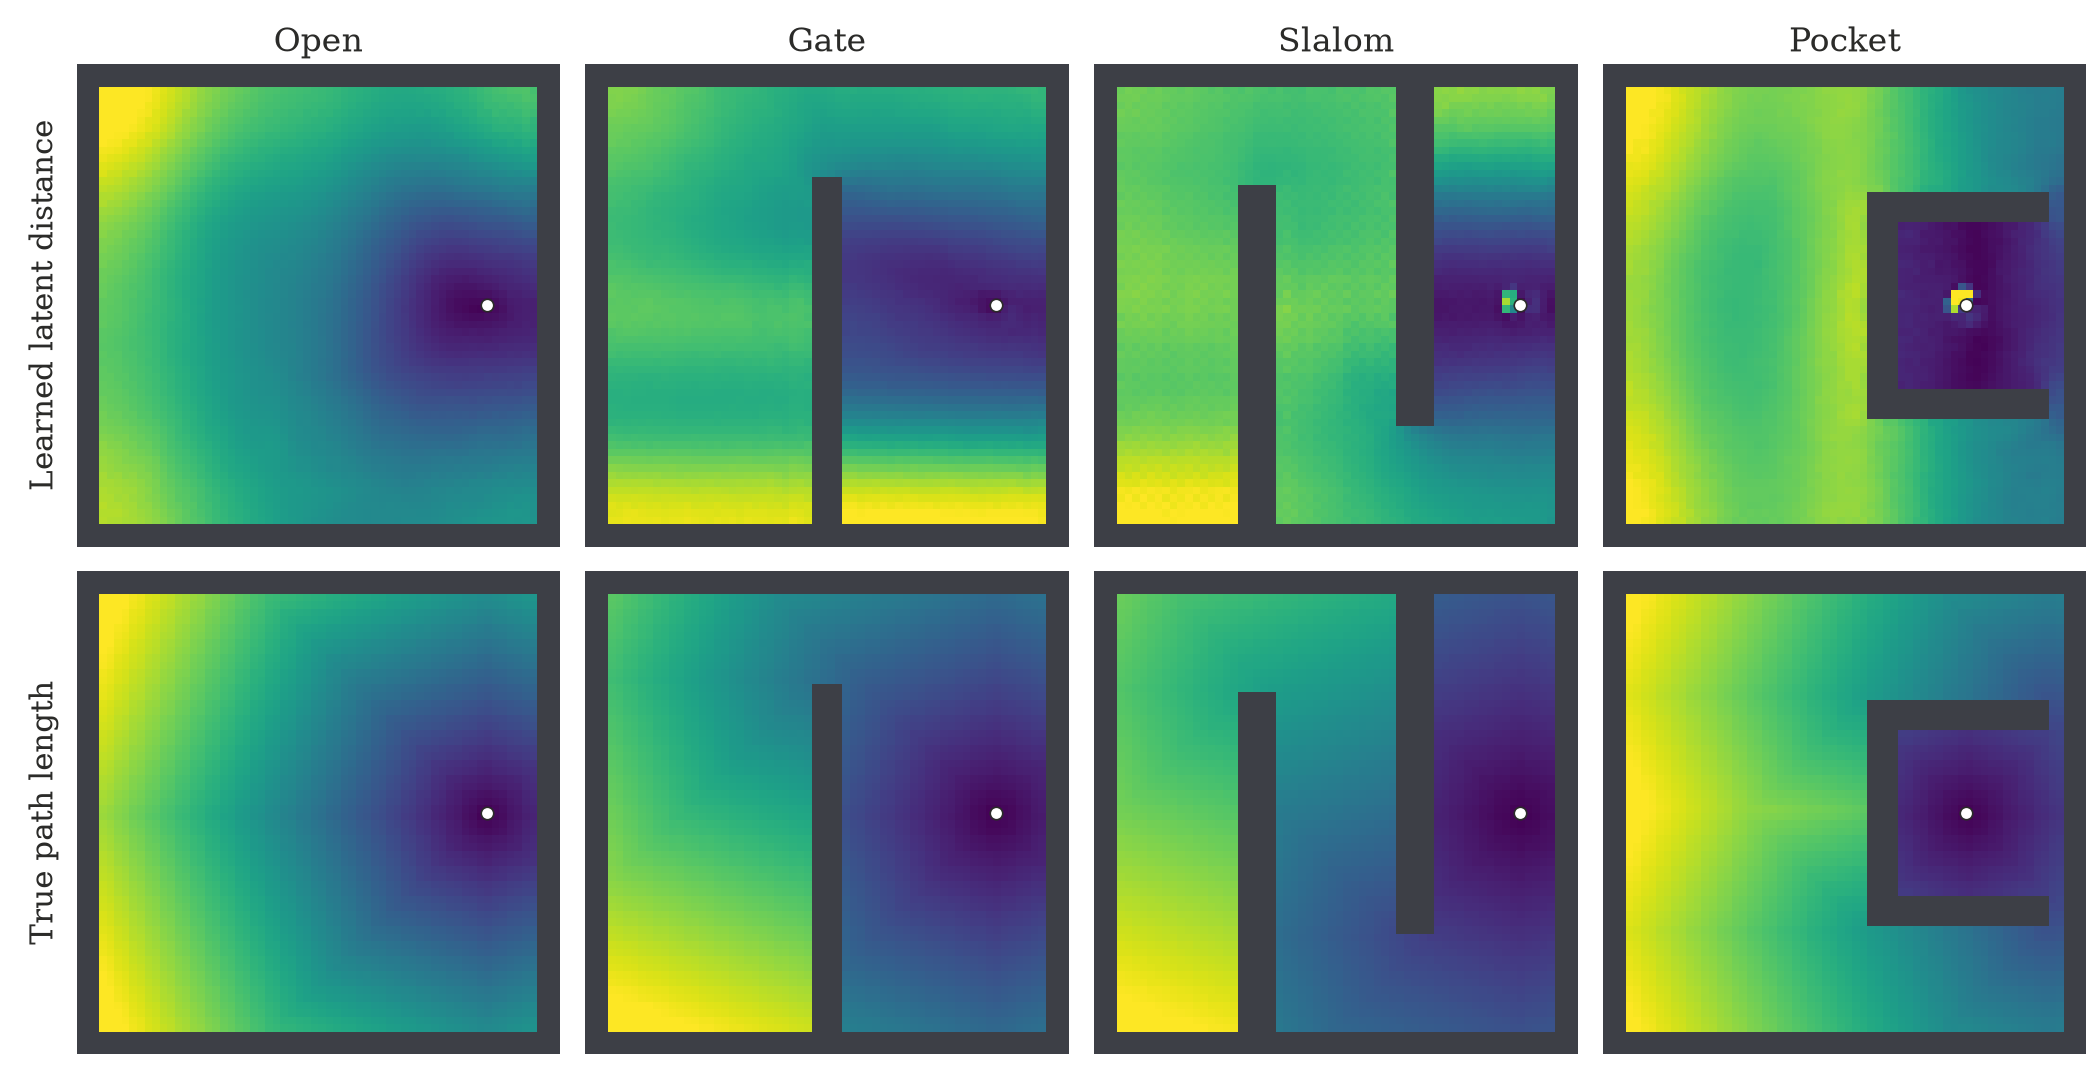
\includegraphics[width=\linewidth]{distance_maps.png}\\[0.25em]
\small A small LeWorldModel saw only random shots as $64\times64$ images: no rewards, no rules, no wall positions.
Top row: its learned distance to the hole. Bottom row: the true path length.
\end{frame}
\begin{frame}{Shots reveal the walls, not the picture}
\begin{columns}[T]
\column{0.5\textwidth}
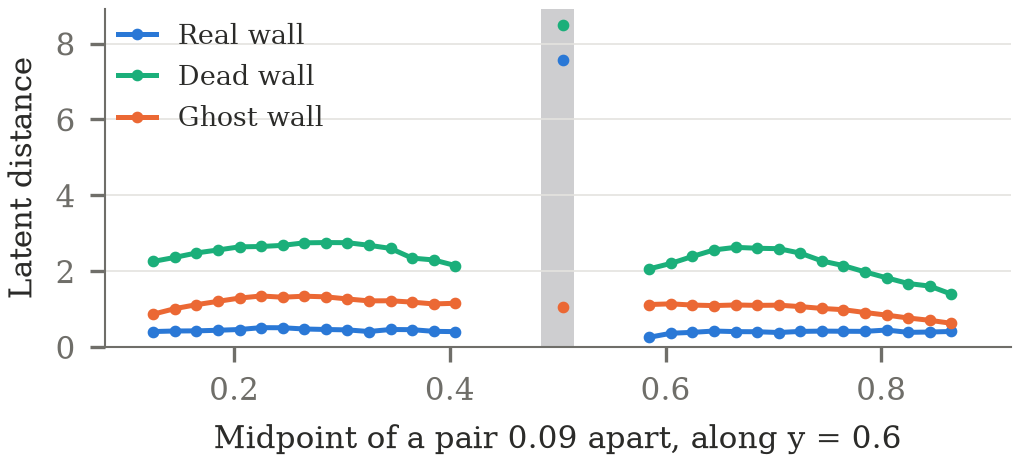
\includegraphics[width=\linewidth]{wall_profile.png}\\[0.4em]
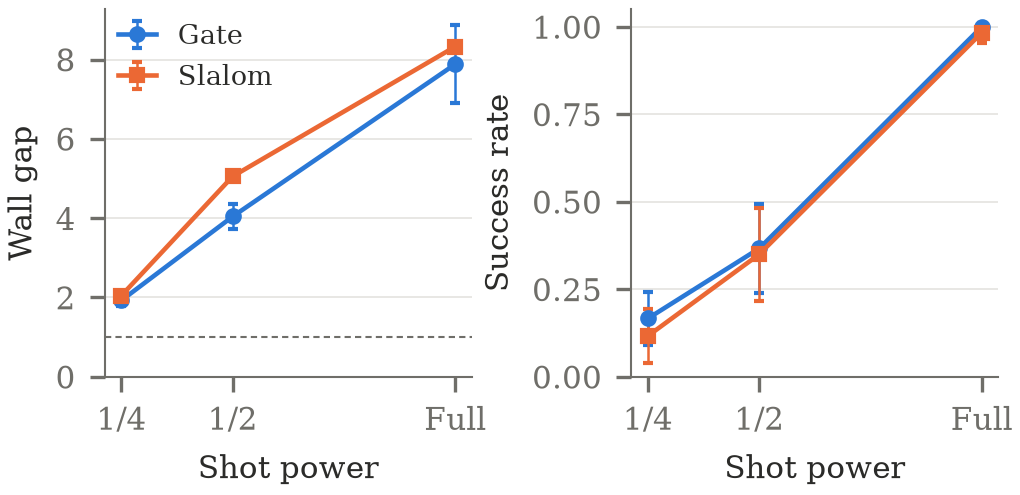
\includegraphics[width=\linewidth]{power.png}
\column{0.48\textwidth}
\small
\begin{itemize}
\item A \textbf{ghost wall} is drawn in every image, but the ball rolls through it.
\item Wall gap: \textbf{7.88} real, \textbf{3.82} blocks without bouncing, \textbf{0.96} ghost (1 means no wall).
\item Weaker shots hit walls less, and the wall fades: 7.88, 4.04, 1.93 on Gate.
\item Planning with this distance sinks 97--100\% on Gate and Slalom.
\item Pocket fails (48\%) because of the predictor: true physics with the same cost gets 100\%. My graph planner gave no clear gain.
\end{itemize}
\end{columns}
\end{frame}
\end{document}
